\section{Introduction} \label{sec:intro}


\begin{table}
\begin{tabular*}{\columnwidth}{|l|p{0.76\columnwidth}|}
\hline
\bf Symbol		& \bf Meaning \\\hline
$QR_{q,R}$		& Range query from $q$ to all $o_i : d_{q,o_i} \leq R$) \\\hline
$Q_{s,t}$		& \spath query from $s$ to $t$ \\\hline
$\chi_{s,t}$		& The frequency of a \spath \\\hline
$P_{s,t}$		& A \spath from s to t \\\hline
$d_{s,t}$		& The \spath distance of a path $P_{s,t}$ \\\hline
$\mathfrak{d}_{s,t}$	& $\| t - s \|_2$, the euclidean distance \\\hline
$\mathcal{O}$		& The set of $\poi \in \mathbf{V}$, the set of vertices\\\hline
$o_i$			& Element i in $\mathcal{O}$ \\\hline
$\mathcal{O}_{q,R}$	& The result set of  $o_i \in Q_{q,R}$ \\\hline
$dist_{\mathcal{O}}$	& Table of distances between vertexes $v_s, v_t \in P_{s,t} :  P_{s,t} \in \spath_q$ \\\hline
$\spath_{q}$		& A set of \spath from q to all $o_i$ \\\hline

$\mathcal{QL_R}$	& Query log of range search queries \\\hline
$\Psi$ 			& The Cache \\\hline
% $|SP|$			& Length of a \spath \\\hline
% $|\Psi|$		& Number of vertexes in the cache \\\hline
% $\Phi(sp)$		& The set of all sub-paths in a \spath $sp$ \\\hline
% $\Phi^c(\Psi)$		& The set of all unique (sub-)paths in $\Psi$ \\\hline
% $\Gamma(\Psi)$		& Calculates the total utility of the content in the cache \\\hline 
$G\mathbf{(V,E)}$ 	& Graph representation of the Map \\\hline 
% $\mathbf{V}$ 		& The set of vertexes in the Map \\\hline 
% WL			& Historical workload \\\hline
\end{tabular*}
\caption{Table of Symbols}
\label{tab:symbols}
\end{table}

\begin{algorithm}[bht]
\dontprintsemicolon
\SetVline

\SetKwInOut{Input}{input}\SetKwInOut{Output}{output}\SetKw{Return}{return}

\Input{

	$(q,R)$: A Range query\;
	$\mathcal{O}$: A set of POI \;
}

\Output{

	A set \poi $\in \mathcal{O}$ \;
}

 \funcc{Naive}{(q,R), \mathcal{O}}
{
    \ForEach{$o_i \in \mathcal{O}$}
    {
      \If{$P_{q,o_i} \in \Psi$} 
      { 
	  insert $o_i$ into $result$ \;
      }
      Call \spath API on $Q_{q,o_i}$ \tcp{\emph{\spath from q to $o_i$}} \;
      \If{$d_{q,o_i} \leq R$} 
      {
	  insert $o_i$ into $result$ \; 
      }

    }
    \Return{result} \;
}

\caption{Naive Algorithm}
\label{alg:naive}
\end{algorithm}


\begin{algorithm}[bht]
\dontprintsemicolon
\SetVline

\SetKwInOut{Input}{input}\SetKwInOut{Output}{output}\SetKw{Return}{return}

\Input{

	$(q,R)$: A Range query\;
	$\mathcal{O}$: A set of POI \;
}

\Output{

	A set \poi $\in \mathcal{O}$ \;
}

\funcc{Fair}{(q,R), \mathcal{O}}
{
    \ForEach{$o_i \in \mathcal{O} : \mathfrak{d}_{q,o_i} \leq R$}
    {
      $candidate_{\mathcal{O}} \leftarrow o_i$ \;
    }
    result $\leftarrow$ \naivens((q,R), $candidate_{\mathcal{O}}$) \;

    \Return{result} \;
}

\caption{Fair Algorithm}
\label{alg:fair}
\end{algorithm}


\begin{align}\label{eq:chinaive}
\chi_{s,t}  = | \{ t :\;  QR_{s,R} \in \mathcal{QL_R}, t \in \mathcal{O}, R \in \mathbb{R}, t \in P_{s,t} \} |
\end{align}

\begin{align}\label{eq:chifair}
\nonumber \chi_{s,t}  = | \{ t :\;  QR_{s,R} \in \mathcal{QL_R}, \{t \in \mathcal{O} | \mathfrak{d}_{s,t} \leq R \}, & &\\
R \in \mathbb{R}, \exists P_{s,t} | d_{s,t} \leq R \} | &
\end{align}




\begin{definition}{Range Search}\\
A range search query, denoted by $Q_{q,R}$ consist of a source vertex $q$ and a range $\mathbf{R}$.
The result of $Q_{q,R}$, denoted $\mathcal{O}_{q,R}$, is a set of objects $o_i \in \mathcal{O}$ with \spath distance $d_{s,t} \leq R$ on graph $G\mathbf{(V,E)}$.
\end{definition}


\begin{definition}{Range Search Query Log ($\mathcal{QL_R}$)}\\
A range search query log $\mathcal{QL_R}$ is a collection of timestamped queries that have been issued by users in the past.
A query is on the form $(q,R)$, where $q$ is a query point and $R$ is a range. The full form of the log, $\mathcal{QL_R}$,  is then: $\{(q_0,R_0),\dots,(q_i,R_i)\}$
\end{definition}


Using a query log, $\mathcal{QL_R}: \{(q_0,R_0),\dots,(q_i,R_i)\}$, we first need to expand each query into its \spath result set containing \spaths from $q$ to each \poi reachable within R distance on a road network. 
To find the result set of a query we use one of two algorithms: \naive or \fairns.

The \naive algorithm will not only find the result set of \spath for each query $\in \mathcal{QL_R}$, but also the \spath from $q$ to all other possible \poins, before pruning and returning the result set of \poisns.
\naive does so by first finding all paths from $q$ to any \poi in the cache. Afterwards it will issue \spath queries from $q$ to the remaining \pois not already found via the cache. 
Once all paths are found \naive will prune the set of paths such that only the paths with distance < $R$ remain. This is the result so \naive returns it to the user.

The idea behind the \fair algorithm (see alg. \ref{alg:fair}) is to prune \poisns, which can not belong to the result set of a query, before doing range search. The \fair algorithm works by, for a query (q,R), first finding the set {\it tmp\poins}, of \pois which lay within euclidean distance $R$ of the query point $q$. \fair then invokes the \naive algorithm using {\it tmp\poins} as the set of \poins.
The pruning method of \fair is correct as the euclidean distance $R$ is also the longest \spathns, with length $R$, possible. It is however important to note that this pruning technique only work if the weights of edges in a road network are distances.

Equation \ref{eq:chinaive} and \ref{eq:chifair} define the frequency of a \spath in $\Psi$, using \naive or \fair respectively.

An Example of how \fair might work is shown in fig. \ref{fig:queryreg}. In it we have 2 queries: $q_1$ and $q_2$. Each query have a range $R=13$ associated with it, which is used to form the pruning areas (circles) of the queries. The pruning areas are the shown by the 2 circles, each covering a query. The  white circles are all vertices. $v_1,\ldots,v_{11}$ are the regular vertices. $o_1,\ldots,o_{10}$ represent the \poisns, and $q_1,q_2$ are the query points. Vertices ($\mathbf{V}$), and connecting lines,edges ($\mathbf{E}$), model a road network, $G\mathbf{(V,E)}$.

In our problem the range $R$ is constrained on a road network, meaning that after pruning, when the vertexes more than $R$ euclidean distance away are no longer considered, the remaining vertexes may still be further than $R$ distance in the road network. 
We can see an example of this with $q_2$, where only one out of the 3 \poi in the gray region is actually within $R$ \spath distance ($o_9$, the reader should visually easily be able to confirm this using the edge weights in fig \ref{fig:queryreg}).

When we consider what to put into the cache, then we will include \spaths for all \poi within the pruning area, regardless of whether the \pois are contained in the result set or not. The reasoning behind this, is that if we only add the exact result, then we will not be able to determine if the entire result is in the cache or not, except in the special case that all vertexes in the pruning region is part of the result, as with query $q_1$.

% To illustrate how we use the cache we will assume $q_1,q_2,$ and $q_3$ have all been executed and \spathsns, from their query points to the \pois in their respective pruning regions, have been added to the cache.
% When $q_4$ is executed then we will first do the pruning to reduce the vertexes we consider. Then we check the cache for any \spath which contains the vertex of $q_4$, which it does in this case, namely the path from $q_1$ to $q_4$. We don't actually need the \spath them selves, but we need their distances (retrieved from $dist_{\mathcal{O}}$) to check whether the \pois are in the result or not, without invoking the \spath API.



% \begin{figure}[hbt]
%   \center
%         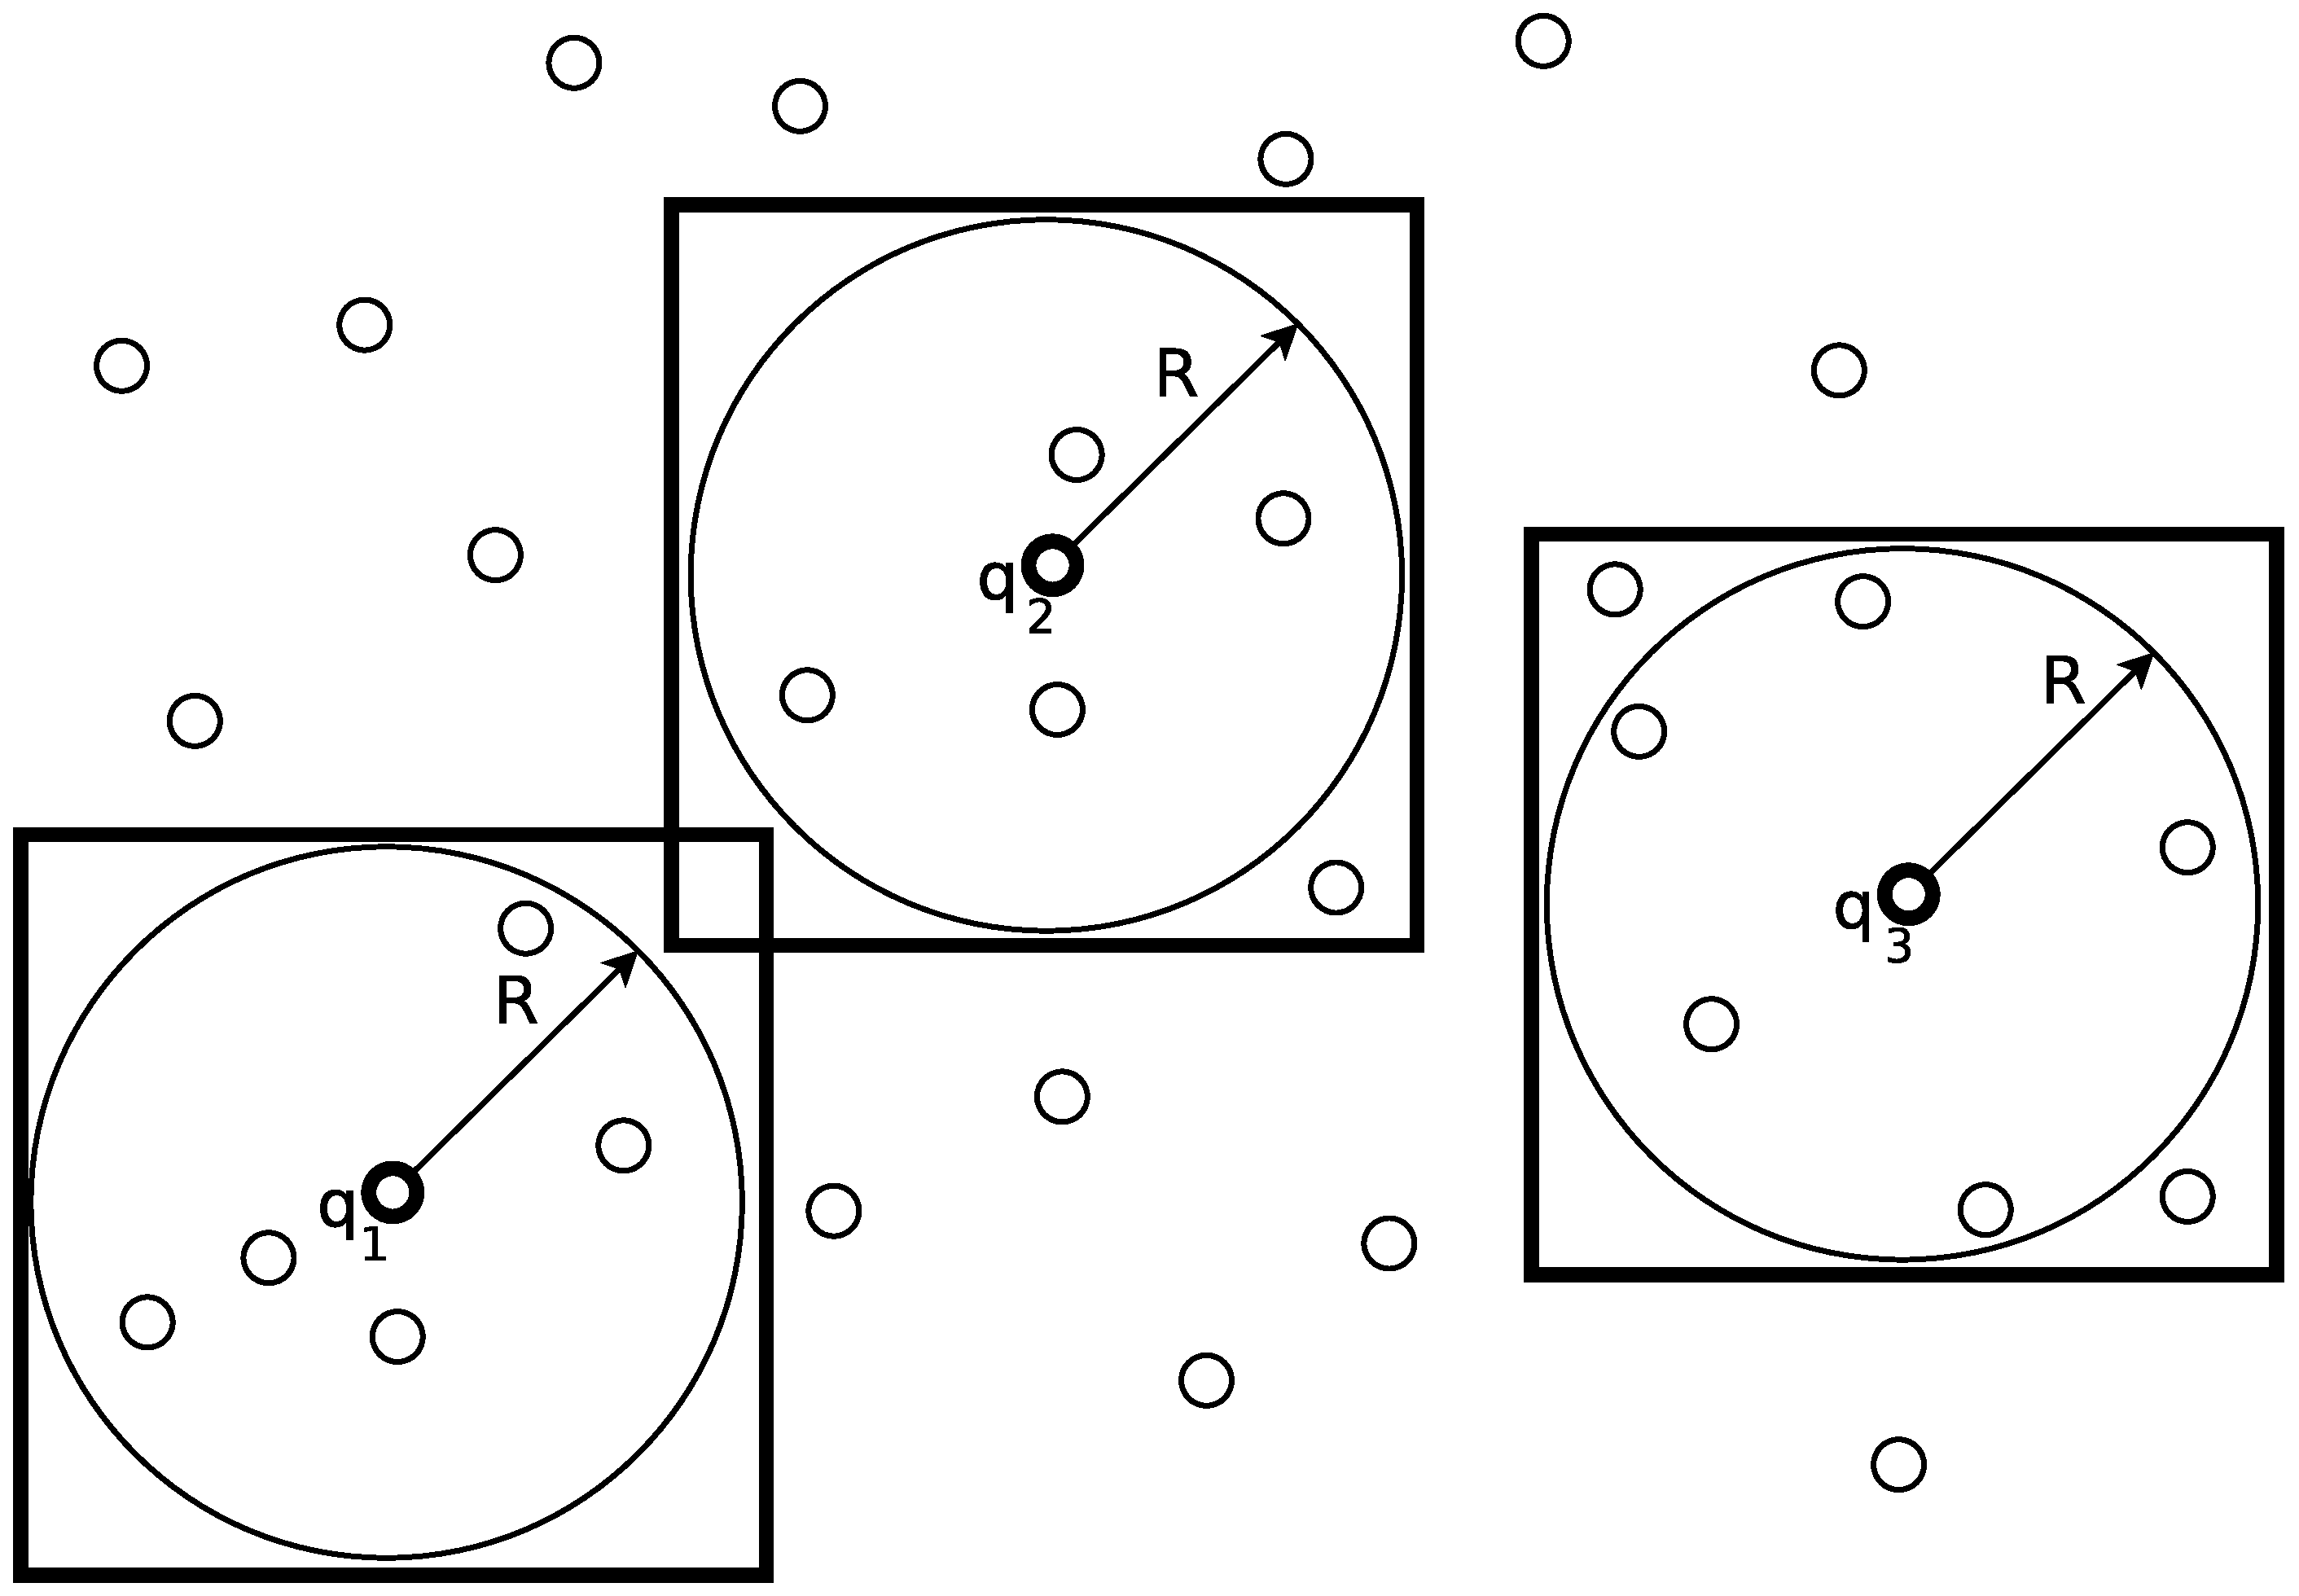
\includegraphics[width=0.5\textwidth]{figures/queryregions}
%         \caption{Query points $q_1,q_2,q_3$, with region defined by R. White points are \poins}
%   \label{fig:queryreg}
% \end{figure}

\begin{figure}[hbt]
  \center
        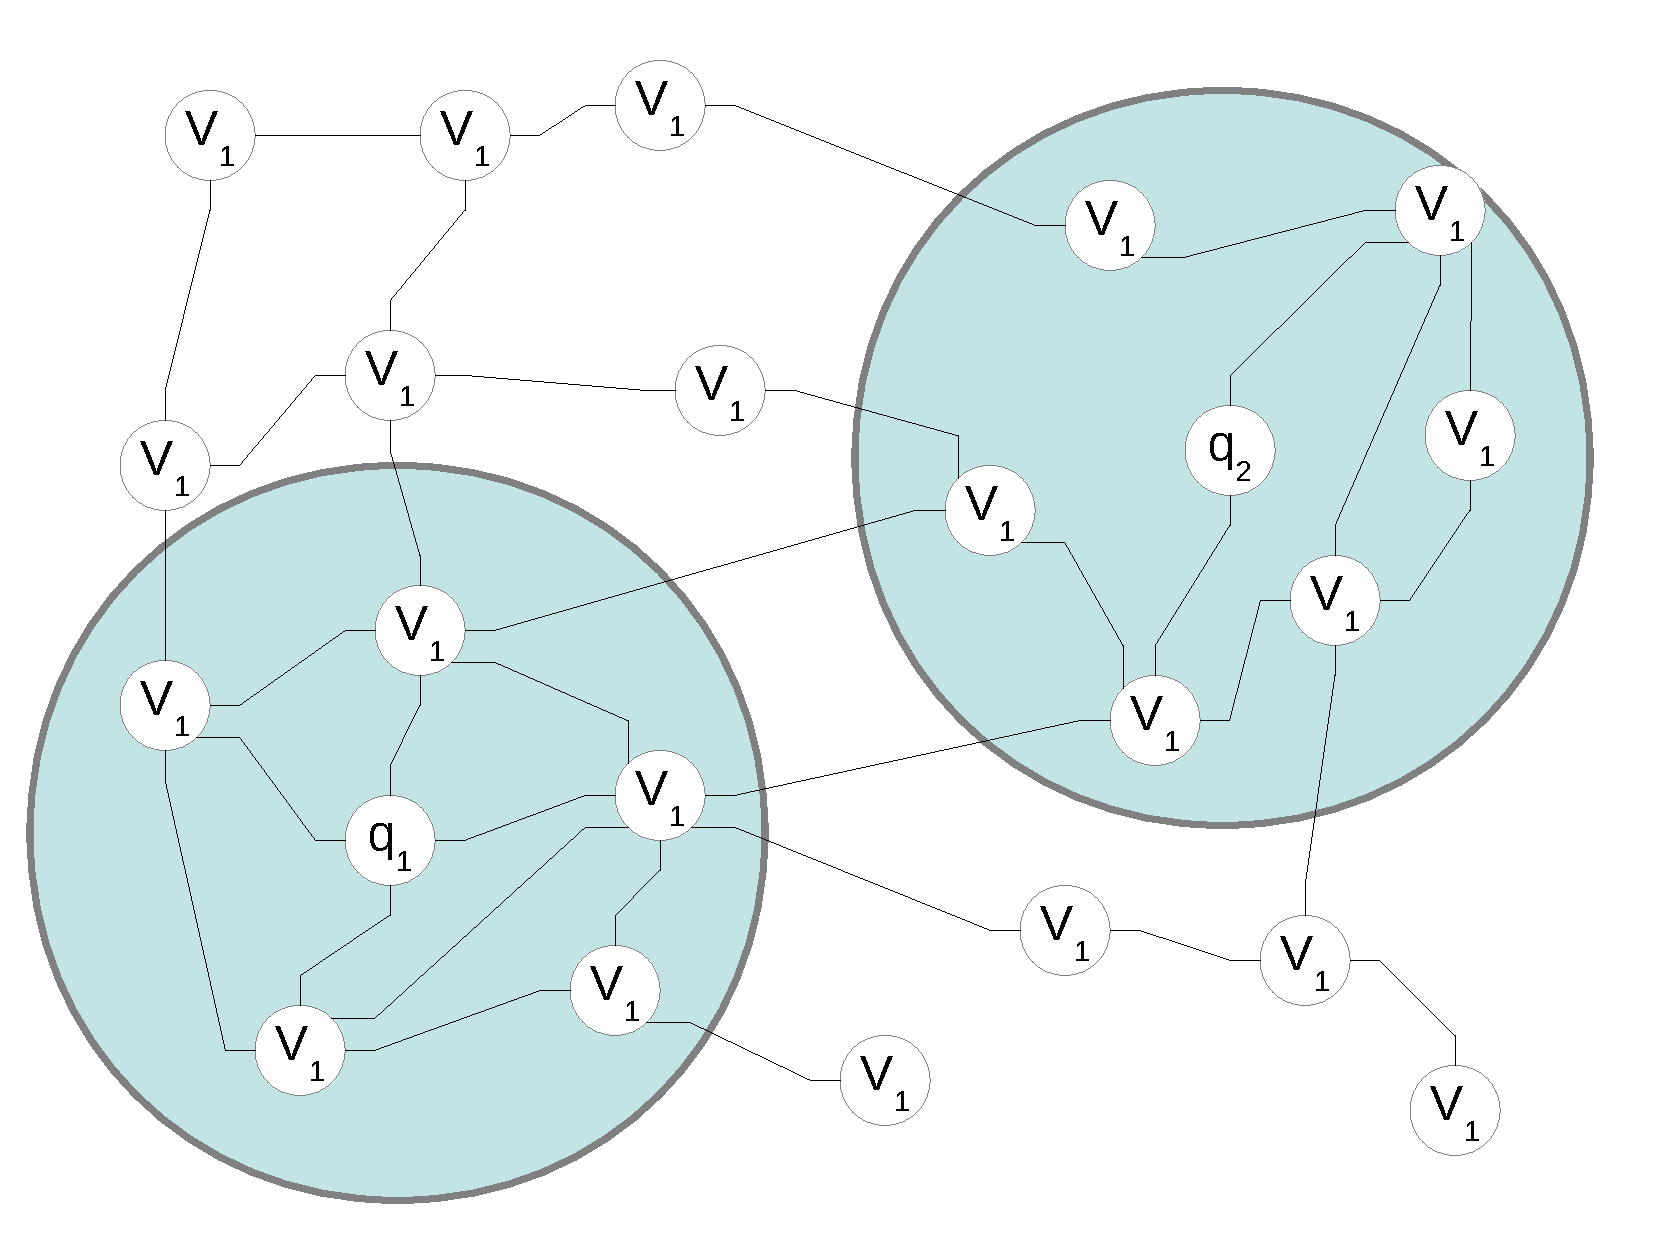
\includegraphics[width=0.5\textwidth]{figures/queryreg}
        \caption{Query points $q_1,q_2,q_3$, with region defined by R. White points are \poins}
  \label{fig:queryreg}
\end{figure}
